\section{Теория}
Уравнение движения твердого тела:
    \begin{equation}
        \frac{\overrightarrow{dp}}{dt}=\overrightarrow{F}
    \end{equation}
    
    \begin{equation}
        \frac{\overrightarrow{dL}}{dt}=\overrightarrow{M}
    \end{equation}
    
    Так как сила $\overrightarrow{F}$ не зависит от угловой скорости, а момент сил $\overrightarrow{M}$ - от скорости поступательного движения, то уравнения движения можно рассматривать отдельно.
    \begin{equation}
        \overrightarrow{L}=\overrightarrow{i}I_x\omega_x+\overrightarrow{j}I_y\omega_y+\overrightarrow{k}I_z\omega_z
    \end{equation}
    
    Гироскоп  - быстро вращающееся тело, для которого, например:
    \begin{equation}
        I_z\omega_z\gg I_x\omega_x, I_y\omega_y
    \end{equation}
    
    Уравновешенный гироскоп - тот, у которого центр масс неподвижен.
    Если момент внешних сил действует в течение короткого промежутка времени, то:
    \begin{equation}
        \left|\Delta \overrightarrow{L}\right|=\left|\int \overrightarrow{M}dt\right|\ll \left|\overrightarrow{L}\right|
    \end{equation}
    
    Рассмотрим маховик, вращающийся вокруг оси $z$ (рис. \ref{маховик}). Будем считать, что:
    \begin{equation}
        \omega_x=\omega_0,\quad		\omega_y=0, \quad	\omega_z=0
    \end{equation}
    
    \begin{figure}[h!]
        \begin{center}
        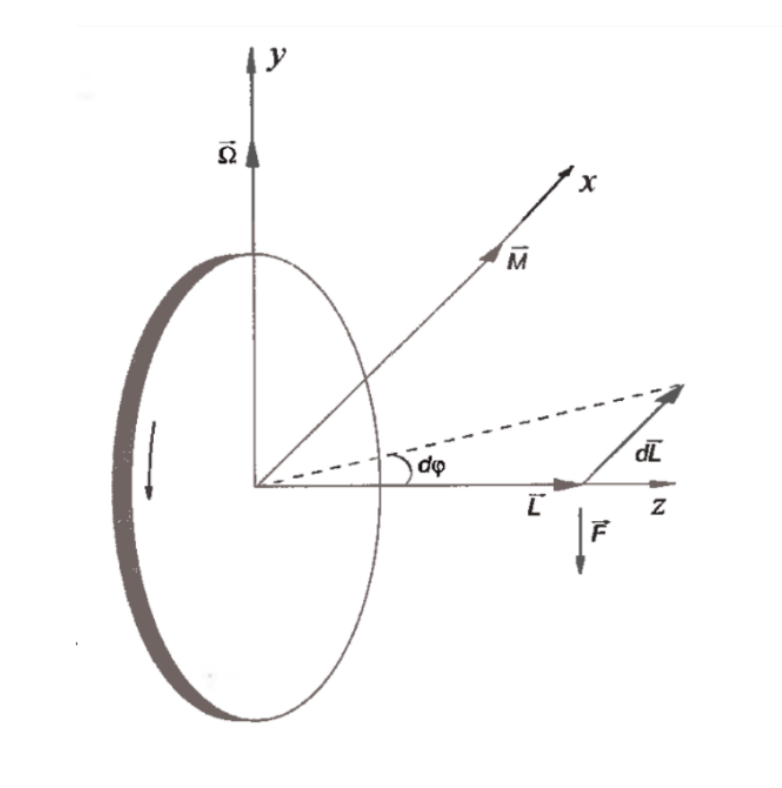
\includegraphics[width=0.4\textwidth]{./images/1.png}
        \end{center}
        \caption{Маховик} \label{маховик}
    \end{figure}
    
    Пусть ось вращения повернулась на угол $d\varphi$ в плоскости $zx$:
    \[d\varphi=\Omega dt\]
    Будем считать, что $L_\Omega \ll \L_{\omega_0}$ 
    Это означает, что момент импульса маховика изменится только по направлению:
    \begin{equation}
        \left|\overrightarrow{dL}\right|=Ld\varphi=L\Omega dt
    \end{equation} 
    
    Изменение направлено вдоль оси x, поэтому $\overrightarrow{dL}$ можно представить:
    \begin{equation}
        \frac{\overrightarrow{dL}}{dt}=\overrightarrow{\Omega}\times\overrightarrow{L}
    \end{equation}
    
    С учетом уравнения вращательного движения:
    \begin{equation}
        \overrightarrow{M}=\overrightarrow{\Omega}\times\overrightarrow{L}
    \end{equation}
        
    Под действием момента $\overrightarrow{M}$ ось гироскопа медленно вращается вокруг оси $y$ с угловой скоростью $\Omega$ - регулярная прецессия гироскопа.
    Скорость в случае движения уравновешенного гироскопа под действием моментов сил подвешенных грузов:
    \begin{equation}
        \label{связь омег}
        \Omega = \frac{mgl}{I_z\omega_0},
    \end{equation}
    
    где $l$ - расстояние от центра карданова подвеса до точки крепления груза на оси гироскопа (рис. \ref{схема})
    \begin{figure}[h!]
        \begin{center}
        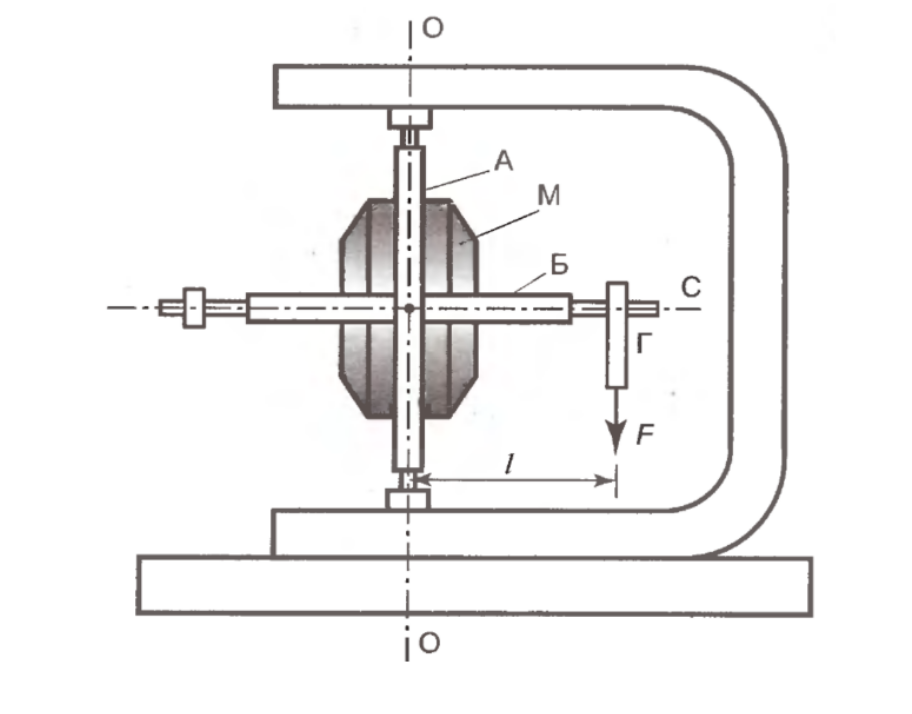
\includegraphics[width=0.5\textwidth]{./images/2.png}
        \end{center}
        \caption{Схема экспериментальной установки} \label{схема}
    \end{figure}
    
    
    Силы трения не лежат в плоскости осей вращения, поэтому они могут изменять момент импульса и по направлению, и по величине. Для ротора действие сил трения скомпенсировано действием электромотора. В результате действия нескомпенсированных сил трения в осях карданова подвеса ось гироскопа будет опускаться в направлении груза.
    
    Момент инерции ротора относительно оси симметрии $I_0$ измеряется по крутильным колебаниям на жесткой проволоке. 
    
    \begin{equation}
        T_0 = 2\pi\sqrt{\frac{I_0}{f}},
    \end{equation}
    
    где $f$ - модуль кручения проволоки
    Чтобы исключить $f$ можно подвесить цилиндр с известными размерами и массой:
    \begin{equation}
        I_0 = I_\text{ц}\frac{T_0^2}{T_\text{ц}^2}
    \end{equation}